\section{Data System Architecture}
\begin{figure}[H]
    \centering
    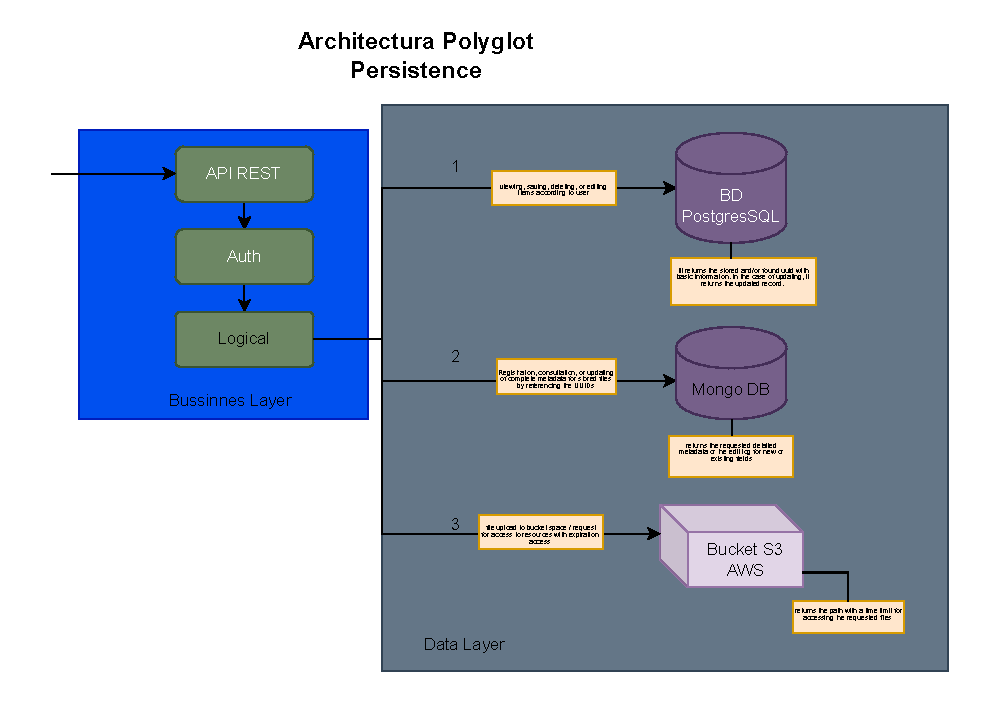
\includegraphics[width=\linewidth, height=0.4\textheight, keepaspectratio]{initialdbarch/architecture_diagram.pdf}
    \caption{Architecture High Level Model for the File Storage Platform.}
    \label{fig:architecture_diagram}
\end{figure}
The system implements a Polyglot Persistence Architecture designed for a cloud-based file storage system (Dropbox-like), optimizing data management through specialized database technologies. The architecture follows a three-tier model with clear separation of concerns between the Business Layer and Data Layer.

\subsection{Component Roles in the Flow}
\subsection{Logical Orchestrator}
Provides advanced workflow management across several data stores and acts as the focal point for all multi-step procedures. File type whitelist validation, file size restriction enforcement, and user storage quota verification are among the business rules enforced by this component. The orchestrator coordinates sequential operations across PostgreSQL, MongoDB, and S3 while preserving compensating transaction logic for rollback circumstances by implementing the SAGA pattern for distributed transaction management. In order to provide end-to-end request tracing across all system components, this component creates distinct correlation identifiers for every action.
\subsection{PostgreSQL Database}
plays two roles in the sequence of data flow. As the authoritative source of records in Step 1, PostgreSQL creates first file records with status='PENDING' and generates unique file identifiers (UUID v4). This first entry creates the file's presence in the system and stops it from showing up in user interfaces until the upload is finished. By using database-level constraints to ensure referential integrity, the database preserves important relational structures, such as foreign key relationships between users, folders, and files. Step 4: PostgreSQL completes the last state transition by changing the file status from 'PENDING' to 'COMPLETED' and storing the S3 storage key. This essentially commits the distributed transaction and makes the file accessible to users.
\subsection{MongoDB Database}
Serves as the adaptable metadata repository, holding variable-structure metadata documents that vary greatly depending on the type of file. Without the need for foreign key constraints, each MongoDB object makes reference to the file-id produced by PostgreSQL, creating a logical relationship. Nested, hierarchical metadata structures, such as EXIF data for photos, codec information for films, and extracted text for documents, are all expertly stored by MongoDB. Rapid feature development is made possible by the schema-less design, which only involves inserting documents with more metadata fields rather than requiring schema changes. Full-text search across extracted material, tag-based filtering, and sophisticated metadata searches are all supported by MongoDB's extensive query language.
\subsection{AWS S3 Bucket}
It employs a key-value storage model in which each file is represented by a unique object key, enabling scalable and efficient management of binary data. AWS S3 automatically handles geographic replication, high availability (99.99\% SLA), and exceptional data durability (99.999999999\%), ensuring continuous access and data resilience. The key naming encodes hierarchical organization while guaranteeing global uniqueness through the \texttt{file\_id} component. Moreover, S3’s pre-signed URL mechanism allows secure, direct client-to-storage data transfers, removing the application server from the critical download path and improving system throughput. Its built-in versioning functionality preserves historical file states, facilitating rollback operations and ensuring compliance with data retention policies.
\subsection{Justification of Technologies}
\textbf{PostgreSQL} was selected as the primary relational database management system due to its robustness, reliability, and advanced support for structured data. It provides strict data integrity through ACID compliance, which is essential for managing critical entities such as user accounts, authentication, access control, and transactional operations. The relational schema allows the definition of complex relationships and constraints, ensuring data consistency and enforcing referential integrity across users, permissions, and file ownership. Additionally, PostgreSQL’s support for stored procedures, indexing, and JSON fields offers the flexibility to handle semi-structured data without compromising performance or normalization principles.

\textbf{MongoDB} complements the relational model by managing unstructured and highly variable data, particularly the metadata associated with stored files. Since each file may contain distinct attributes depending on its type (e.g., images, videos, documents), MongoDB’s document-oriented architecture enables dynamic schema evolution without the need for rigid table structures. This flexibility allows for rapid scaling and efficient querying of metadata at high volumes, while maintaining strong integration with the application layer through native JSON compatibility. Furthermore, MongoDB’s sharding and replication capabilities ensure horizontal scalability and data redundancy, which are crucial for a cloud-based storage system.

\textbf{Amazon S3 (Simple Storage Service)} was chosen as the core object storage solution to handle the actual file data independently of the databases. S3 provides virtually unlimited, durable, and cost-effective storage with built-in redundancy across multiple availability zones. By decoupling file storage from metadata management, the architecture optimizes both performance and scalability. Files are stored in S3 buckets, while their metadata and relational references are maintained in MongoDB and PostgreSQL, respectively. This separation of concerns enhances security, simplifies data retrieval, and supports advanced features such as access versioning, encryption, and temporary file-sharing links — all essential for a professional-grade file storage platform.
